\documentclass[11pt,letterpaper]{article}
\usepackage[lmargin=1in,rmargin=1in,bmargin=1in,tmargin=1in]{geometry}
\usepackage{quiz}

% -------------------
% Content
% -------------------
\begin{document}
\thispagestyle{title}

% Quiz 1
\quizsol \textit{True/False}: The expression $12 \div 6 \cdot 2 + (-1)^3$ is the same as $\frac{12}{6 \cdot 2} + (-1)^3$ and both are equal to $0$. \pspace

\sol The statement is \textit{false}. We can compute both, following order of operations (PEMDAS, applied carefully left-to-right), and show that the expressions evaluate to different values:
	\[
	\begin{gathered}
	12 \div 6 \cdot 2 + (-1)^3 \\
	12 \div 6 \cdot 2 - 1 \\
	2 \cdot 2 - 1 \\
	4 - 1 \\
	3
	\end{gathered} \hspace{4cm}
	\begin{gathered}
	\tfrac{12}{6 \cdot 2} + (-1)^3 \\
	\tfrac{12}{6 \cdot 2} - 1 \\
	\tfrac{12}{12} - 1 \\
	1 - 1 \\
	0
	\end{gathered}
	\]
For these two expressions to be the same, the first needs a set of parentheses around the $6 \cdot 2$: $12 \div (6 \cdot 2) + (-1)^3$. \pvspace{1.3cm}



% Quiz 2
\quizsol \textit{True/False}: The point $(2, -6)$ is in the third quadrant and is a distance of 2 away from the $x$-axis and a distance of $6$ away from the $y$-axis. \pspace

\sol The statement is \textit{false}. Because $x= 2 > 0$ and $y= -6 < 0$, the point $(2, -6)$ is in Quadrant~IV. Moreover, plotting the point $(2, -6)$, we can see that the point is a distance of $|2|= 2$ away from the $x$-axis and a distance of $|-6|= 6$ away from the $y$-axis. 
	\[
	\fbox{
	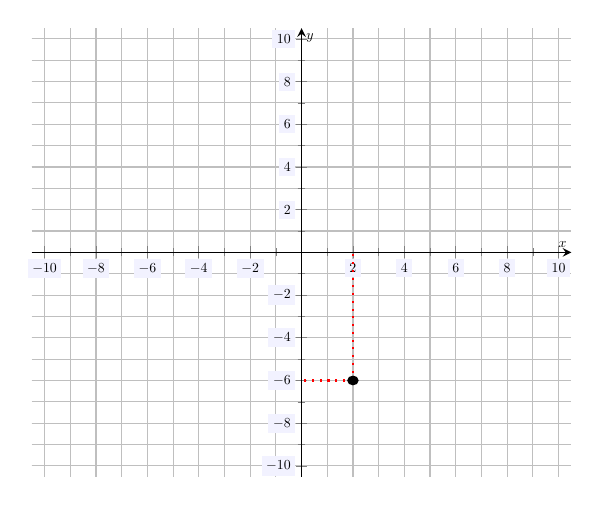
\begin{tikzpicture}[scale=1,every node/.style={scale=0.5}]
	\begin{axis}[
	grid=both,
	axis lines=middle,
	ticklabel style={fill=blue!5!white},
	xmin= -10.5, xmax=10.5,
	ymin= -10.5, ymax=10.5,
	xtick={-10,-8,-6,-4,-2,0,2,4,6,8,10},
	ytick={-10,-8,-6,-4,-2,0,2,4,6,8,10},
	minor tick = {-10,-9,...,10},
	xlabel=\(x\),ylabel=\(y\),
	]
	\draw[dotted,thick,red] (2,-6) -- (0,-6);
	\draw[dotted,thick,red] (2,-6) -- (2,0);
	\draw[fill=black] (2,-6) circle (0.2);
	\end{axis}
	\end{tikzpicture} 
	}
	\] \pvspace{1.3cm}



% Quiz 3
\quizsol \textit{True/False}: The average rate of change of a function is the quotient of the change in output by the change in input. If the average rate of change is positive, the function increased. If the average rate of change is negative, the function decreased. \pspace

\sol The statement is \textit{true}. We know that the average rate of change of a function $f(x)$ over the interval $[a, b]$ is given by $\frac{f(b) - f(a)}{b - a}$. Because $x$'s are the inputs and $f(x)$'s are the outputs, this is $\frac{\Delta \text{output}}{\Delta \text{input}}$. Now because $b > a$, we know that $b - a > 0$. So the sign of the average rate of change depends only on the sign of $f(b) - f(a)$. If $f(b) - f(a) > 0$, then $f(b) > f(a)$. But then the function increased in value from the value at $x= a$ to the value at $x= b$. If $f(b) - f(a) < 0$, then $f(b) < f(a)$. But then the function decreased in value from the value at $x= a$ to the value at $x= b$. Neither imply that the function was increasing or decreasing, respectively, over the \textit{entire} interval $[a, b]$. \pvspace{1.3cm}



% Quiz 4
\quizsol \textit{True/False}: The average rate of change of a function $f(x)$ on an interval $[a, b]$ is the slope of the secant through the points $\big(a, f(a) \big)$ and $\big(b, f(b) \big)$. \pspace

\sol The statement is \textit{true}. We know that the average rate of change of a function $f(x)$ over the interval $[a, b]$ is given by $\frac{f(b) - f(a)}{b - a}$. Given the points $\big(a, f(a) \big)$ and $\big(b, f(b) \big)$, the slope of the line through them is $m= \frac{\Delta y}{\Delta x}=  \frac{f(b) - f(a)}{b - a}$. 
	\[
	\fbox{
	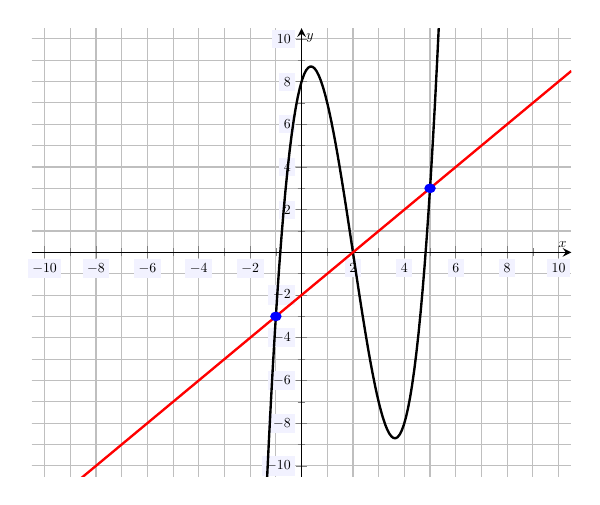
\begin{tikzpicture}[scale=1,every node/.style={scale=0.5}]
	\begin{axis}[
	grid=both,
	axis lines=middle,
	ticklabel style={fill=blue!5!white},
	xmin= -10.5, xmax=10.5,
	ymin= -10.5, ymax=10.5,
	xtick={-10,-8,-6,-4,-2,0,2,4,6,8,10},
	ytick={-10,-8,-6,-4,-2,0,2,4,6,8,10},
	minor tick = {-10,-9,...,10},
	xlabel=\(x\),ylabel=\(y\),
	]
	\addplot[line width=0.03cm, domain= -2:6,samples=100] ({x},{x^3 - 6*x^2 + 4*x + 8});
	\addplot[line width=0.03cm, domain= -9:10.5,samples=2,red] ({x},{x - 2});
	\draw[fill=black,blue] (-1,-3) circle (0.2);
	\draw[fill=black,blue] (5,3) circle (0.2);
	\end{axis}
	\end{tikzpicture} 
	}
	\] \pvspace{1.3cm}



% Quiz 5
\quizsol \textit{True/False}: If $P(t)= 5300t - 1480$ is a linear model representing the population in a small town $t$~years from now, then $m= 5300 > 0$ means that the model says that the population is growing at a rate of 5,300 people per year. Furthermore, the $y$-intercept $b= 1480$ represents the exact initial population of the town. \pspace

\sol The statement is \textit{false}. We know that the function $P(t)$ is linear, i.e. the graph of $P(t)$ is a line. We know that $m= 5300$. Recalling that $m= \frac{\Delta P}{\Delta t}$ and writing $5300= \frac{5300}{1}$, we can see that for every one increase in $t$ results in a 5300 increase in $P$, i.e. the population is growing at a rate of 5,300~people per year. Of course, this is just what the model says happens, on average. The $y$-intercept is $P(0)= 5300(0) - 1480= -1480$. But then $b \neq 1480$. Because $b= P(0)= -1480 < 0$, this cannot possibly represent a population. Furthermore, $b= P(0)$ need not represent the \textit{exact} initial population, merely what the model predicts is the initial population. 


























\end{document}